In this simulation, we have tested the performance in terms of gain in the SNR at the output of the five
 beamformers we have implemented for:

\begin{enumerate}
    \item Different number of interfering signals
    \item Different values of SNRs at the input of the beamformers
\end{enumerate}

\subsection{Geometry and parameters}

We are using a $LOS$ channel in stationary conditions (vehicles are not moving). The vehicles are positioned at a 
distance of 25 meters from the base station on a circumference and spaced of $\ang{20}$ as in Figure \ref{fig:Scenario_circle}. \\ 
The antenna array we are using is a 4x4 array.

\begin{figure}[ht]
    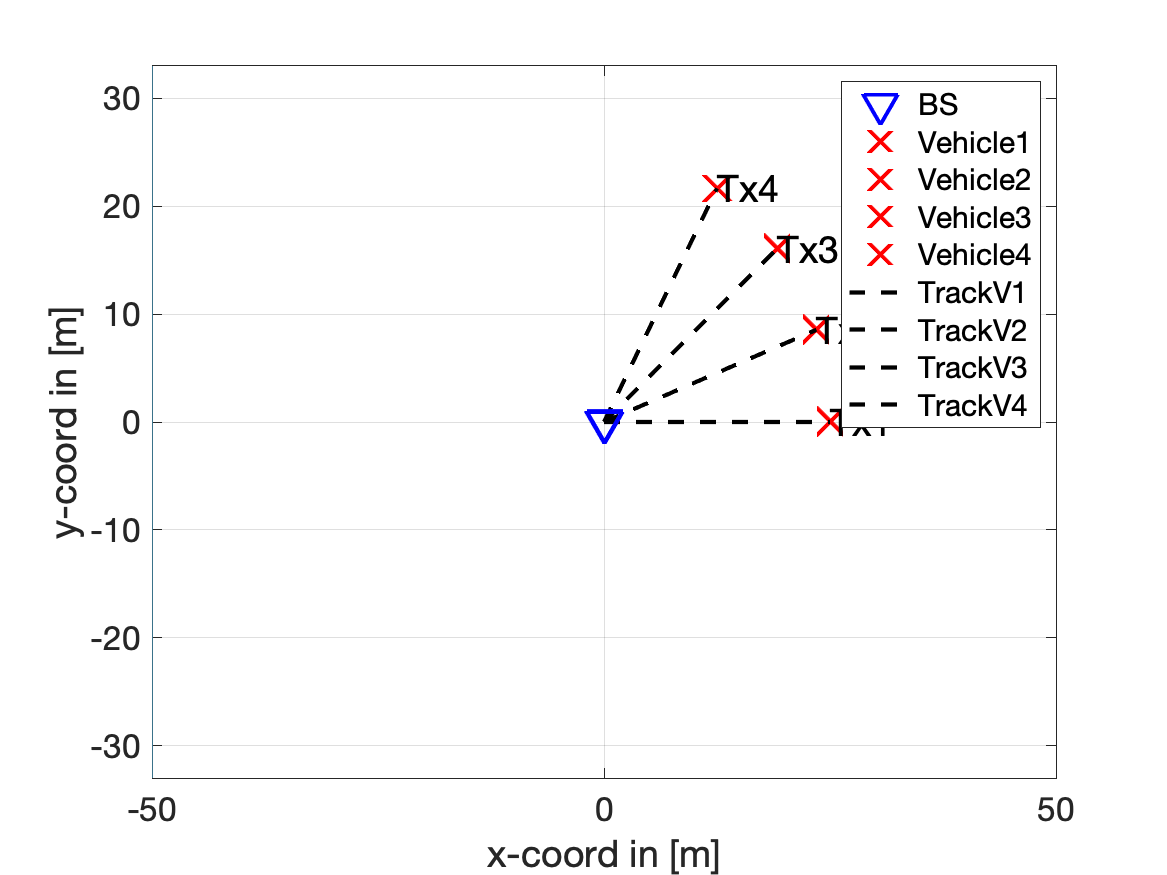
\includegraphics[width=\linewidth]{Scenario_circle.png}
    \caption{Scenario of the simulation}
    \label{fig:Scenario_circle}
\end{figure}

\subsection{Steps of the simulation}

Our simulation considers a different number of interferents (0, 1, 2, 3) and for each one of the cases computes the 
curve input SNR - output SNR for all the beamformers:

\begin{enumerate}
    \item Definition of the current number of interferents
    \item Generation of the scenario and of the singnals
    \item Passage of signals through the $LOS$ channel
    \item For all the input SNR levels:
    \begin{enumerate}
        \item Add noise to the good signal in a way that the SNR is the current one
        \item Computation of the weights of the antenna elements 
        \item Application of beamforming techniques to the single signals and noise
        \item Computation of the power of all the signals and of the noise
        \item Computation of the SNR at the output of the beamformers
    \end{enumerate}
    \item Plot of the results
\end{enumerate}

\subsection{Results}

In Figure \ref{fig:SNR_comparison}, we can see in the four graphs the curves SNRin - SNRout. In a single figure, the 
number of interferents is fixed and we show the lines for the different beamformers.

\begin{figure}[ht]
    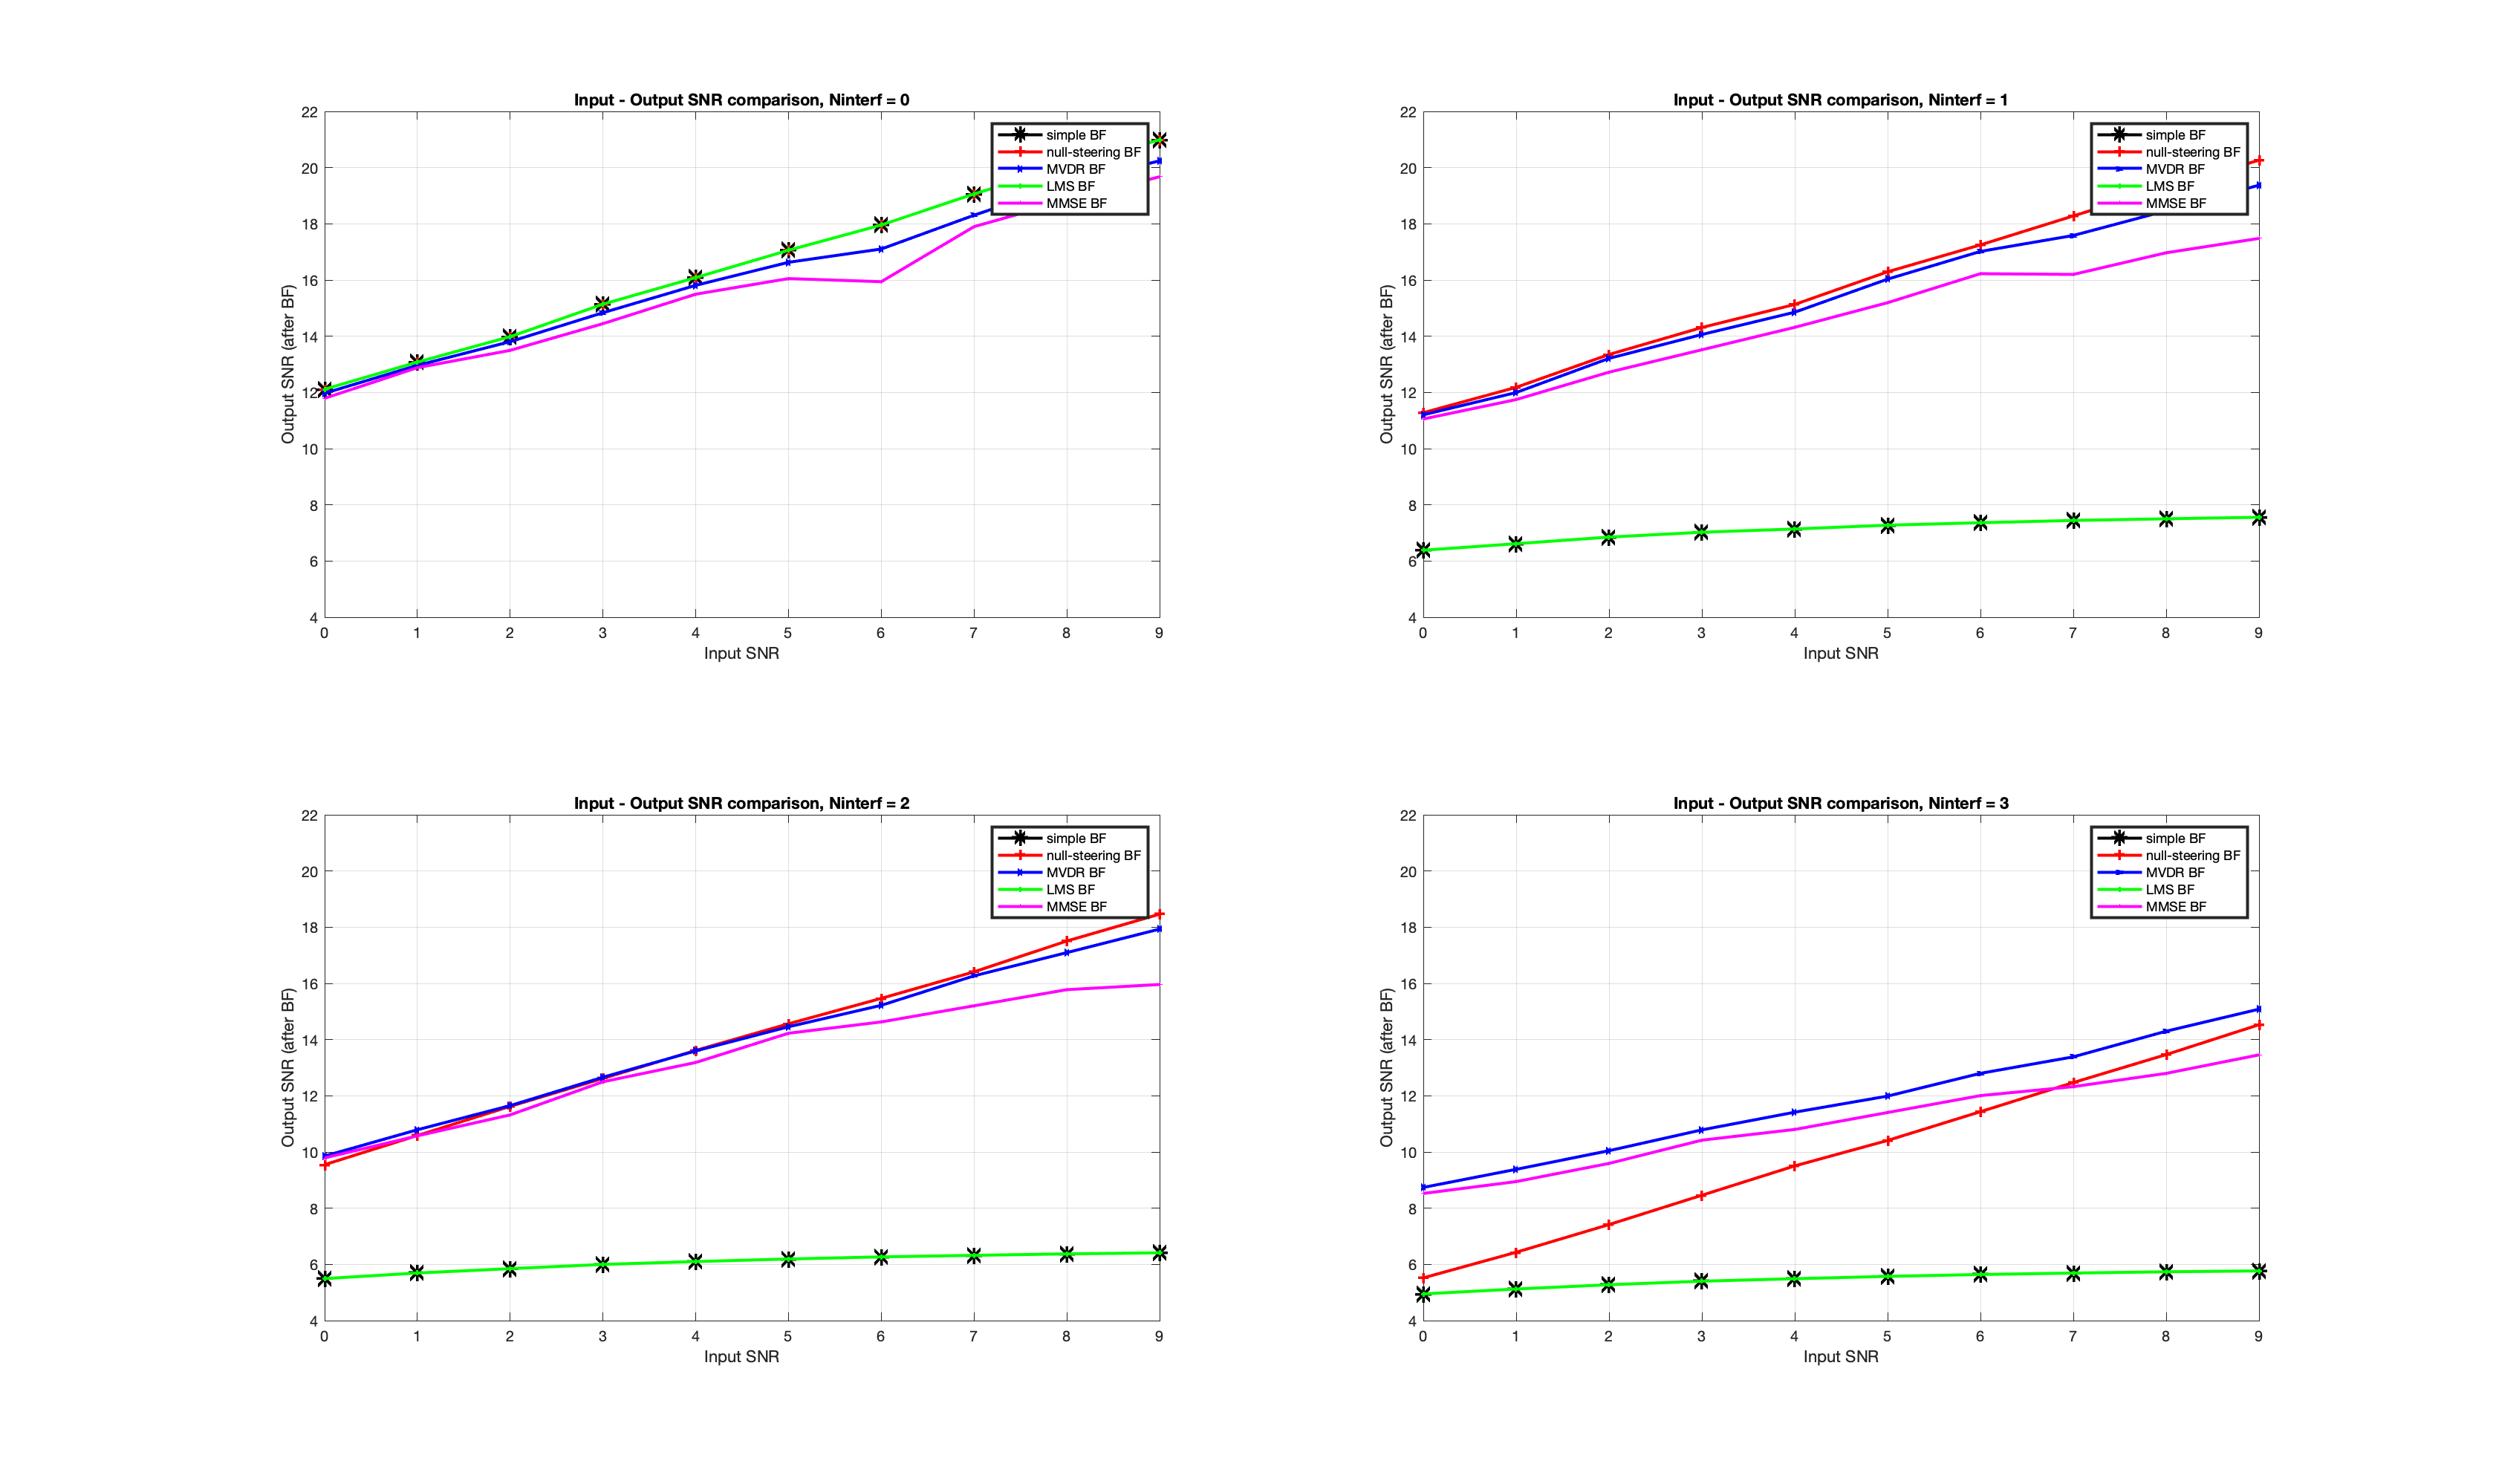
\includegraphics[width=\linewidth]{SNR_comparison.png}  
    \caption{Relation SNRin - SNRout for different interfering signals and beamformers (LMS initialized with simple BF)}  
    \label{fig:SNR_comparison}
\end{figure}

As we can see, without any interfering signals, the behavior of all the beamformers is almost linear and the gain is 
approximately constant and equal to 12dB.\\ 
As the number of interferents increases, we can identify as general behavior:

\begin{enumerate}
    \item The simple and the LMS beamformer are the worst one; indeed, their curves are the most bended and the 
            ones giving the lowest gain. This is expected for the simple beamformer and, in this case, also for the LMS
            since we are initializing its state using the simple beamformer. This is not the best choice (and
            in fact the gain of the LMS is low), but its a simple way of initializing it.
    \item The MVDR and the MMSE are the beamformers that behaves better since they are designed for minimizing respectively the 
            interference-plus-noise power at the beamformer output and the error with respect to a reference singal. Anyway, as 
            the number of interferents increases their gain decreases, but still their curves are almost linear. 
    \item The null-steering beamformer behaves as the MVDR and the MMSE with for 0, 1 or 2 interfering signals, but its gain
            decreases with three interferents. This is due to the fact that this beamformer tries to put a null in correspondence
            of the DoA of the interferents and, in case there are too many ones and too close one to each other, this becomes 
            difficult and the gain decreases.
\end{enumerate}